\chapter{Learning Rules With Numerical and Categorical Attributes}
\label{cl:intro}

In this chapter we will discuss what kind of rules we are interested in, define what categorical properties are,
describe in more details a \graphname, how to build it and integrate it in the core ILP learning algorithm.

\section{Interesting Rule Definition}
%\label{cl:interestingRules}

In this section we formally define what kind of rules we are interested in obtaining with the algorithm proposed in
this thesis. As briefly explained in the introduction, the objective is to learn rules with numerical properties,
focusing on searching ranges in the numerical attribute's domain that satisfy support and confidence thresholds.

Searching numerical intervals for a base-rule that already satisfies confidence threshold is not so interesting. The
base-rule itself implicitly specifies an interval which covers the whole numerical attribute domain from any possible
refined-rules. Moreover, even if for some specific range we have a higher confidence value, the gain in comparison to
the base-rule would not be so great as the base-rule already present a high confidence value (at least higher than the
specified threshold).

More precisely, if we have a confidence threshold $TS_{conf}$ and defining confidence gain from a refined-rule
$r_2$ in comparison to a base-rule $r_1$ as $g_{r_2,r_1}$ as:

\begin{equation}
 g_{r_2,r1}=\cfrac{conf_{r_2}}{conf_{r_1}}
\end{equation}

As we know that $r_1 \geq TS_{conf}$, then $g_{r_2,r_1}$ is upper-bounded by:

\begin{equation}
 g_{r_2,r1} \leq \cfrac{1}{TS_{conf}}
\end{equation}

More interesting for us would be base rules that satisfy the support threshold but does not satisfy the confidence
threshold. In such case, if we have a non-uniform confidence distribution along the buckets, it's possible for some
intervals, its correspondent refined-rule satisfies both thresholds. Furthermore, the confidence gain is potentially
much greater than otherwise.
 
\section{Categorical Property Definition}

In this section, we formally define a categorical property as used in the \graphname. 

First of all, a candidate relation must be joined with root relation's non-numerical variable

A candidate categorical relation $r(x,y)$, should be equivalent to a non-injective function:

$r(x,y) \equiv f : X \rightarrow Y , \quad s.t. \quad |Y|<|X| $ and $ |Y|>1 \newline $
Therefore, $\nexists \, g : Y \rightarrow X , \quad s.t. \quad f(g(x))=x , \quad \forall x \in X$

We can define subsets $X_i \in X$, with which $X_i$ belonging to one category $y_i \in Y$:

$X_i \subset X \quad s.t. \quad X_i = \{x \in X \,|\, f(x)=y_i ,\, y_i \in Y\} \newline $
$X = \bigcup_{i=1}^{n} X_i $ and $ X_i \cap X_j = \emptyset ,\quad \forall i,j \in [1,n] ,\, i \neq j$

We can also broaden this definition by composing functional relations with a categorical or multiple categorical
relations:

If we have:

$r_1(x,y) \equiv f_1 : X \rightarrow Y$ \newline
$r_2(y,z) \equiv f_2 : Y \rightarrow Z$ 

Where at least one of them is categorical, then $r'(x,z) \equiv f : X \rightarrow Z$, where $r'(x,z)=r_2(f_1(x),z)$ is also categorical


Numerical properties can also be turned into a categorical, by simply applying a bucketing function that maps a
numerical domain into a finite set of $k$ buckets:

$b: \mathbb{N} \rightarrow B$, where $B=\{1,2,\dots ,k \}$

e.g.: [make an example]

So a numerical property:

$r(x,y) \equiv f : X \rightarrow \mathbb{N}$ 

combined with a bucketing function $b$, $r'(x,b(y))$ would be discretized and applicable in the \graphname.

Types are also covered by this definition. If we consider \emph{r = rdf:type} we see that $r$ which maps entities into
types satisfies the definition presented before.

Similarly different knowledge bases can be interconnected by simply applying this definition with the \emph{owl:sameAs}
relation. This allows to broaden the set of categorical properties to be analyzed in the \graphname to those contained
in interlinked datasets.

\subsection{Absence or Presence of a Property as Categories}

Another possibility is to define categories for presence or absence of supporting examples for properties. With this
approach, one can also
include non-categorical properties into the \graphname and have insight about how the presence or absence of such
property affects the distribution of root's numerical attribute.

In this case we must consider a property which doesn't have examples for all its domain. For example, the property
\emph{isParentOf(x,y)} has as both domain and range type Person. If not all the Person instances of the knowledge base
have supporting facts for the relation \emph{isParentOf}, then we can
split the instances in two categories: the ones that are covered by the property and the ones that are not. For example,
let \emph{hasIncome} be the root property and let's assume we have a knowledge base with the following facts:

\begin{tabular}{*{2}{l}}
  hasIncome(John,20000) & isParentOf(John,Mary) \\
  hasIncome(Mike,30000) & isParentOf(Mike,Paul) \\
  hasIncome(Anne,25000) & isParentOf(Anne,Paul) \\
  hasIncome(Mary,5000) 	& isParentOf(Anne,Mary) \\
  hasIncome(Lisa,10000) & 			\\
  hasIncome(Paul,0)	& 			\\
\end{tabular}

Then we could split the root node set $X_{root}=\{x|\exists hasIncome(x,z)\}$ in two categories $X_{root}^1,X_{root}^2
\in
X_{root}$:

$X_{root}^1=\{x| x \in X_{root} \land \exists isParentOf(x,y)\} \\$
$X_{root}^2=\{x| x \in X_{root} \land \nexists isParentOf(x,y)\} \\$

Each group would consist of the following instances:

$X_{root}=\{John,Mike,Anne,Mary,Lisa,Paul\} \\$
$X_{root}^1=\{John,Mike,Anne\} \\$
$X_{root}^2=\{Mary,Lisa,Paul\}$

As in this thesis we are under open world assumption and we don't consider negated literals in the hypothesis, we ignore
the absence and just include the presence of relations in the lattice.


\subsection{Notation Used}

As we will see in the next sections, in the \graphname all the relations are joined by the variable of root's first
argument. So we will denote the presence of a property $r(x,y)$ category as simply $r$, where $x$ is the join variable
and $y$ is free and not set to any constant. If we have a categorical property $a(x,y)$ with $k$ different categories
$A_i \in Y$ $(i=1,..,k)$, we denote each of the $a(x,A_i)$ as $a_i$.

So if we have a root node $r$ and a node at level 3 called $rab_1c_3$, that means we are considering the examples for
the following join:

$r(x,y)a(x,z)b(x,B_1)c(x,B_3)$


\section{Preprocessing}

In this section, we will present the preprocessing steps required by our proposed algorithm. It basically consists of
first building a joinable relations map for each join pattern, according
to relations domain and range types as well as support threshold. Afterwards, we search the available categorical
properties for each numerical relation that will be used in the \graphname. At last we build the so called \graphname,
which belongs to the preprocessing step but will be discussed in the next section.

\subsection{Relation Preprocessing}

In this step, we focus on creating a map of joinable for each join pattern between two relations. As in this thesis we
are working with RDF triples, we have four possible join patterns:

\begin{itemize}
 \item Argument 1 on Argument 1: e.g. \emph{hasIncome(\textbf{x},y)hasAge(\textbf{x},z)}
 \item Argument 1 on Argument 2: e.g. \emph{hasIncome(\textbf{x},y)isMarriedTo(z,\textbf{x})}
 \item Argument 2 on Argument 1: e.g. \emph{livesIn(y,\textbf{x})isLocatedIn(\textbf{x},z)}
 \item Argument 2 on Argument 2: e.g. \emph{livesIn(y,\textbf{x})wasBornIn(z,\textbf{x})}
\end{itemize}

With that we could easily obtain all the possible pair of joinable relations for each join pattern, avoiding testing
hypothesis containing invalid join pairs.

\subsubsection{Exploiting Relation Range and Domain Types}

A knowledge base is expected to have an ontology defining the structure of the stored data (the types of entities and
their relationships). Additionally, every relation's range (type of \ord{1} argument) and domain (type of \ord{2}
argument) should be defined. These information can help us identify the allowed joining relations for each join pattern.

\begin{figure}[!h]
  \caption{Type hierarchy example}
  \centering
  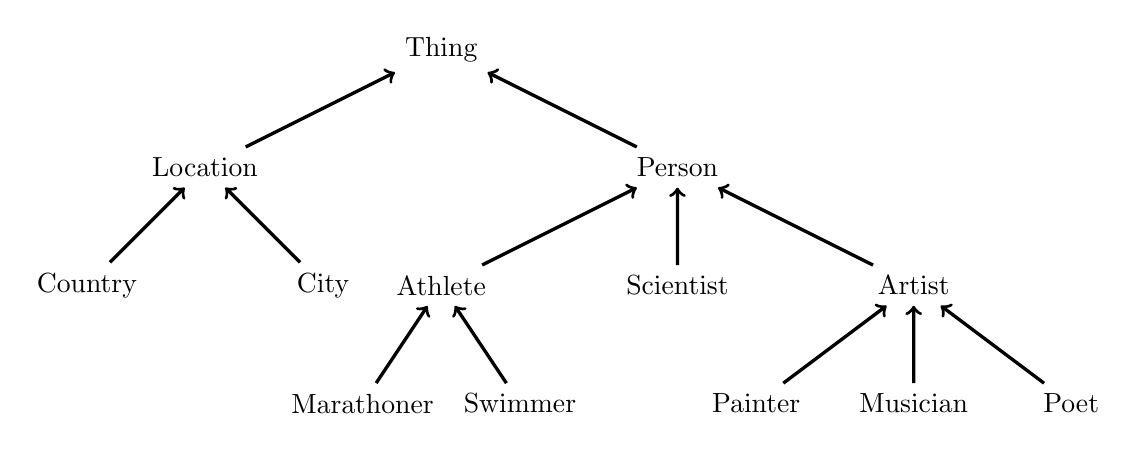
\begin{tikzpicture}[<-,draw=black,very thick,level/.style={sibling distance = 6cm/#1,level distance = 1.5cm}]
    
    \node{Thing}
      child{node {Location} 
	child{node {Country}}
	child{node {City}}
      }
      child{node {Person}
	child{node {Athlete}
	  child{node {Marathoner}}
	  child{node {Swimmer}}
	}
	child{node {Scientist}}
	child{node {Artist}
	  child{node {Painter}}
	  child{node {Musician}}
	  child{node {Poet}}
	}
      };
  \end{tikzpicture}

\label{fig:typeHierarchy}
\end{figure}

Assuming that the knowledge base has its type hierarchy described with the relation \emph{rdfs:subClassOf} and both
argument types from each of the relations declared with \emph{rdfs:domain} and \emph{rdfs:range} it is a
straightforward task.

For every possible pair of relations, we simply try to match the joining argument types from the 2 joining relations. We
check whether they are equal or if one can be subsumed by the other. If so, then it's allowed to join the pair of relations
on the given joining arguments, or in other words, the type hierarchy doesn't prevent them from joining. The pseudo-code
for performing such task is
shown in the Algorithm \ref{alg1}:

\begin{algorithm}[!h]
  \caption{Function $checkTypes$ \newline Checks whether two relations are joinable for a given join pattern}
 \label{alg1}
 \SetKwFunction{subsumes}
 \KwIn{\textbf{Input:} $r_i$, $r_j$: Joining relations, $arg_i$, $arg_j$: Joining arguments \\}
 \KwOut{True if $arg_i$ from $r_i$ joins with $arg_j$ from $r_j$, False otherwise}
  \Switch{$arg_i$} {
      \Case{$1$}{
	$type_i \leftarrow r_i.domain$ \;
      }
      \Case{$2$}{
	$type_i \leftarrow r_i.range$ \;
      }
  }
  \Switch{$arg_j$} {
      \Case{$1$}{
	$type_j \leftarrow r_j.domain$ \;
      }
      \Case{$2$}{
	$type_j \leftarrow r_j.range$ \;
      }
  }
  \eIf{$type_i = type_j$ {\bf or} \FuncSty{subsumes(}$type_i$,$type_j$\FuncSty{)} {\bf or}
       \FuncSty{subsumes(}$type_j$,$type_i$\FuncSty{)}}{
      \Return true\;
   }{
    \Return false\;
  }
\end{algorithm}

Nevertheless, it might be that in the knowledge base, the cardinality of such join might be zero or simply not exceed
the support threshold. Thus, it's worth to that beforehand, and that's what will be explained in the next section.

\subsubsection{Exploiting Support Monotonicity}

Support is a monotonically decreasing measure in top-down ILP. So we know that by adding any
literals to the hypothesis, we can only get a smaller or equal support. Therefore, for each pair of joinable relations
in each of the join patterns, we can query the knowledge base and check whether they have enough supporting facts.

Thus, if any pair of relations doesn't reach the minimum support for a given join pattern, we know that any clause
containing such join will therefore fail the support test as well, so we don't need to test such hypothesis in the core
ILP algorithm.

\begin{algorithm}[!h]
  \caption{Function $checkSupport$ \newline Checks whether join support exceeds threshold}
  \label{alg2}
  \SetKwFunction{executeQuery}
  \KwIn{\textbf{Input:} $r_i$, $r_j$: Joining relations, $arg_i$, $arg_j$: Joining arguments, $supportThreshold$:
Support threshold \\ }
  \KwOut{True if join support exceeds threshold, False otherwise}
    \Switch{$(arg_i,arg_j)$} {
      \Case{$(1,1)$}{
	$query \leftarrow$ \emph{``select count distinct $?x$ where \{ $?x$ <$r_i$> $?y$ . $?x$ <$r_j$> $?z$ \}''} \;
      }
      \Case{$(1,2)$}{
	$query \leftarrow$ \emph{``select count distinct $?x$ where \{ $?x$ <$r_i$> $?y$ . $?z$ <$r_j$> $?x$ \}''} \;
      }
      \Case{$(2,1)$}{
	$query \leftarrow$ \emph{``select count distinct $?x$ where \{ $?y$ <$r_i$> $?x$ . $?x$ <$r_j$> $?z$ \}''} \;
      }
      \Case{$(2,2)$}{
	$query \leftarrow$ \emph{``select count distinct $?x$ where \{ $?y$ <$r_i$> $?x$ . $?z$ <$r_j$> $?x$ \}''} \;
      }
    }
    $joinSupport \leftarrow$ executeQuery($query$)\;
     \eIf{$joinSupport \ge supportThreshold$} {
      \Return true\;
    }{
      \Return false\;
    }
\end{algorithm}


The preprocessing is done by algorithm \ref{alg3}, which applies \ref{alg1} and \ref{alg2} on all the possible join pair
combinations and extracting the valid ones, we can build 4 joining maps, one for each join pattern. Each map has
relations as keys and a set of joinable relations as value. In the refinement step at the ILP algorithm, these maps will
be queried in order to obtain suggestions of literals to be
added.

\begin{algorithm}[!h]
  \caption{Preprocessing algorithm}
  \label{alg3}
  \SetKwFunction{executeQuery}
  \KwIn{\textbf{Input:} $r$: Set of Relations, $supportThreshold$: The support threshold \\ }
  \KwResult{$L_{m,n}(r_i)$: List of joinable relations, where $m,n \in \{1,2\}, r_i \in r$}

    \tcp{Lists initialization}
    \ForEach{$r_i \in r$} {
      $L_{1,1}(r_i) \leftarrow r_i$ \;
      $L_{2,2}(r_i) \leftarrow r_i$ \;
      $L_{1,2}(r_i) \leftarrow \emptyset$ \;
      $L_{2,1}(r_i) \leftarrow \emptyset$ \;
    }
    \tcp{For every possible pair of relations}
    \ForEach{$r_i \in r$} {
	\ForEach{$r_j \in r$ {\bf and} $j \geq i$} {
	    \If{$r_i \neq r_j$} {
		\If{$checkTypes(r_i,r_j,1,1)$ {\bf and} $checkSupport(r_i,r_j,1,1)$} {
		    $L_{1,1}(r_i) \leftarrow L_{1,1}(r_i) \cup r_j$ \;
		    $L_{1,1}(r_j) \leftarrow L_{1,1}(r_j) \cup r_i$ \;
		}
		\If{$checkTypes(r_i,r_j,2,2)$ {\bf and} $checkSupport(r_i,r_j,2,2)$} {
		    $L_{2,2}(r_i) \leftarrow L_{2,2}(r_i) \cup r_j$ \;
		    $L_{2,2}(r_j) \leftarrow L_{2,2}(r_j) \cup r_i$ \;
		}
	    }
	    \If{$checkTypes(r_i,r_j,1,2)$ {\bf and} $checkSupport(r_i,r_j,1,2)$} {
		$L_{1,2}(r_i) \leftarrow L_{1,2}(r_i) \cup r_j$ \;
		$L_{2,1}(r_j) \leftarrow L_{2,1}(r_j) \cup r_i$ \;
	    }
	    \If{$checkTypes(r_i,r_j,2,1)$ {\bf and} $checkSupport(r_i,r_j,2,1)$} {
		$L_{2,1}(r_i) \leftarrow L_{2,1}(r_i) \cup r_j$ \;
		$L_{1,2}(r_j) \leftarrow L_{1,2}(r_j) \cup r_i$ \;
	    }
	}
   }
\end{algorithm}

\subsection{}

\section{\graphname}
\label{ch:lattice}

The idea is to build during preprocessing a graph inspired in the itemset lattice that describes the influence of
different categorical relations on a given numerical attribute's distribution. We call such graph a \graphname.
Comparing to a Itemset Lattice, in a \graphname we have a set of categorical relations (that are joined with root
property) instead of items. In addition, Each node in the graph has an associated histogram with the support
distribution over the root's numerical attribute.

To illustrate the idea, let's analyze a simple real-world example with the \emph{hasIncome} relation. If we have two
categorical relations, one strongly correlated to income, e.g. \emph{hasEducation}, and one uncorrelated (or very weakly
correlated), e.g. \emph{wasBornInMonth}.

Let's assume that for the relation \emph{wasBornInMonth(x,y)} we have the 12 months from the Gregorian Calendar as
constants and for \emph{hasEducation(x,y)} we can have 10 different categorical constants for \emph{y}: ``Preschool'',
``Kindergarten'', ``ElementarySchool'', ``MiddleSchool'', ``Highschool'', ``Professional School'', ``Associate's
degree'', ``Bachelor's degree'', ``Master's degree'' and ``Doctorate degree''. 

It's expected that the income distribution will be roughly the same for people born in any of the months, whereas
for different education levels, e.g. Elementary School and Doctoral Degree, their income distribution are expected to be
different from each other them and different from the overall income distribution.

Based on this idea, we basically check how different categorical relations affect a numerical distribution. Such
information, together with other measures such as support, provides valuable cues on what categorical attributes and
what
categorical constants might be the most interesting to be added to the hypothesis in the core ILP algorithm.

\subsection{Building the Lattice}

We first start with the chosen numerical property. We get all the facts existent for this property, define the buckets
and count the examples producing a frequency histogram.

Subsequently, for the chosen set of categorical relations, we do the same with the examples obtained by joining the root
with each of the categories. For every category we create a node in the lattice with assiciated frequency histogram. We
also each the root as parent node, and add the new nodes as children from the root.

In a further step, we try to join every possible pair of categorical relations and including the constants. For the
given, example with the relations \emph{hasEducation} and \emph{wasBornInMonth} we would then create the nodes:

  \emph{hasIncome(x,y)wasBornInMonth(x,``January''),hasEducation(x,``Preschool'')} \newline
  \emph{hasIncome(x,y)wasBornInMonth(x,``January''),hasEducation(x,``Kindergarten'')} \newline
  \dots \newline
  \emph{hasIncome(x,y)wasBornInMonth(x,``January''),hasEducation(x,``Doctorate Degree'')} \newline

  \emph{hasIncome(x,y)wasBornInMonth(x,``February''),hasEducation(x,``Preschool'')} \newline
  \emph{hasIncome(x,y)wasBornInMonth(x,``February''),hasEducation(x,``Kindergarten'')} \newline
  \dots \newline
  \emph{hasIncome(x,y)wasBornInMonth(x,``February''),hasEducation(x,``Doctorate Degree'')} \newline
 
  \dots \newline

  \emph{hasIncome(x,y)wasBornInMonth(x,``December''),hasEducation(x,``Preschool'')} \newline
  \emph{hasIncome(x,y)wasBornInMonth(x,``December''),hasEducation(x,``Kindergarten'')} \newline
  \dots \newline
  \emph{hasIncome(x,y)wasBornInMonth(x,``December''),hasEducation(x,``Doctorate Degree'')} \newline

This process works just like in an itemset lattice until a predetermined maximum level or until all the
possible combinations are exhausted. Figure \ref{fig:lattice} shows how a \graphname looks like.

\begin{figure}[!h]
  \caption{Correlation Lattice example}
  \centering
  \begin{tikzpicture}
  [scale=1.8,auto=center,every node/.style={circle,fill=black!10,minimum size=1.2cm, font=\tiny}]
  \begin{tikzpicture}
 [scale=1.8,auto=center,every node/.style={minimum, font=\tiny}]
  \node (n0) at (4,10) {$r$};
  \node (na) at (0,8)  {$r a$};
  \node (na1)%[fill=blue!20] 
  at (1,7.5)  {$r a_1$};
  \node (na2)%[fill=blue!20] 
  at (2,7.5) {$r a_2$};
  \node (nb) at (3,8)  {$r b$};
  \node (nb1)%[fill=red!20] 
  at (4,7.5)  {$r b_1$};
  \node (nb2)%[fill=red!20] 
  at (5,7.5)  {$r b_1$};
  \node (nc) at (6,8)  {$r c$};
  \node (nc1)%[fill=green!20] 
  at (7,7.5)  {$r c_1$};
  \node (nc2)%[fill=green!20] 
  at (8,7.5)  {$r c_1$};
  \node (nab) at (0,5)  {$r a b$};
  \node (na1b1)%[fill=magenta!20] 
  at (0.5,4.5)  {$r a_1 b_1$};
  \node (na1b2)%[fill=magenta!20] 
  at (1.0,4.5)  {$r a_1 b_2$};
  \node (na2b1)%[fill=magenta!20] 
  at (1.5,4.5)  {$r a_2 b_1$};
  \node (na2b2)%[fill=magenta!20] 
  at (2.0,4.5)  {$r a_2 b_2$};
  \node (nac) at (3,5)  {$r a c$};
  \node (na1c1)%[fill=cyan!20] 
  at (3.5,4.5)  {$r a_1 c_1$};
  \node (na1c2)%[fill=cyan!20] 
  at (4.0,4.5)  {$r a_1 c_2$};
  \node (na2c1)%[fill=cyan!20] 
  at (4.5,4.5)  {$r a_2 c_1$};
  \node (na2c2)%[fill=cyan!20] 
  at (5.0,4.5)  {$r a_2 c_2$};
  \node (nbc) at (6,5)  {$r b c$};
  \node (nb1c1)%[fill=yellow!50] 
  at (6.5,4.5)  {$r b_1 c_1$};
  \node (nb1c2)%[fill=yellow!50] 
  at (7.0,4.5)  {$r b_1 c_2$};
  \node (nb2c1)%[fill=yellow!50] 
  at (7.5,4.5)  {$r b_2 c_1$};
  \node (nb2c2)%[fill=yellow!50] 
  at (8.0,4.5)  {$r b_2 c_2$};
  \node (nabc) at (2,2)  {$r a b c$};
  \node (na1b1c1)%[fill=black!10] 
  at (2.5,1.5)  {$r a_1 b_1 c_1$};
  \node (na1b1c2)%[fill=black!10] 
  at (3.2,1.5)  {$r a_1 b_1 c_2$};
  \node (na1b2c1)%[fill=black!10] 
  at (3.9,1.5)  {$r a_1 b_2 c_1$};  
  \node (na1b2c2)%[fill=black!10] 
  at (4.6,1.5)  {$r a_1 b_2 c_2$};
  \node (na2b1c1)%[fill=black!10] 
  at (5.3,1.5)  {$r a_2 b_1 c_1$};
  \node (na2b1c2)%[fill=black!10] 
  at (6.0,1.5)  {$r a_2 b_1 c_2$};
  \node (na2b2c1)%[fill=black!10] 
  at (6.7,1.5)  {$r a_2 b_2 c_1$};
  \node (na2b2c2)%[fill=black!10] 
  at (7.4,1.5)  {$r a_2 b_2 c_2$};

  \foreach \from/\to in {na/na1,na/na2,nb/nb1,nb/nb2,nc/nc1,nc/nc2}
    \draw[dashed] (\from) -| (\to);

  \foreach \from/\to in {nab/na1b1,nab/na1b2,nab/na2b1,nab/na2b2}
    \draw[dashed] (\from) -| (\to);

  \foreach \from/\to in {nabc/na1b1c1,nabc/na1b1c2,nabc/na1b2c1,nabc/na1b2c2,nabc/na2b1c1,nabc/na2b1c2,nabc/na2b2c1,nabc/na2b2c2}
    \draw[dashed] (\from) -| (\to);

  \foreach \from/\to in {n0/na1,n0/na2,na1/na1b1,na1/na1b2,na2/na2b1,na2/na2b2,na1/na1c1,na1/na1c2,na2/na2c1,na2/na2c2}
    \draw[blue] (\from) -- (\to);
  \foreach \from/\to in {n0/nb1,n0/nb2,nb1/na1b1,nb1/na2b1,nb2/na1b2,nb2/na2b2,nb1/nb1c1,nb1/nb1c2,nb2/nb2c1,nb2/nb2c2}
    \draw[red] (\from) -- (\to);
  \foreach \from/\to in {n0/nc1,n0/nc2,nc1/na1c1,nc1/na2c1,nc2/na1c2,nc2/na2c2,nc1/nb1c1,nc1/nb2c1,nc2/nb1c2,nc2/nb2c2}
    \draw[green] (\from) -- (\to);
  \foreach \from/\to in {na1b1/na1b1c1,na1b2/na1b2c1,na2b1/na2b1c1,na2b2/na2b2c1,na1b1/na1b1c2,na1b2/na1b2c2,na2b1/na2b1c2,na2b2/na2b2c2}
    \draw[magenta] (\from) -- (\to);
  \foreach \from/\to in {na1c1/na1b1c1,na1c1/na1b2c1,na2c1/na2b1c1,na2c1/na2b2c1,na1c2/na1b1c2,na1c2/na1b2c2,na2c2/na2b1c2,na2c2/na2b2c2}
    \draw[cyan] (\from) -- (\to);
  \foreach \from/\to in {nb1c1/na1b1c1,nb2c1/na1b2c1,nb1c1/na2b1c1,nb2c1/na2b2c1,nb1c2/na1b1c2,nb2c2/na1b2c2,nb1c2/na2b1c2,nb2c2/na2b2c2}
    \draw[yellow] (\from) -- (\to);

  \foreach \from/\to in {n0/na,n0/nb,n0/nc}
    \draw[dashed] (\from) -- (\to);
  \foreach \from/\to in {na/nab,na/nac,nb/nab,nb/nbc,nc/nac,nc/nbc,nab/nabc,nac/nabc,nbc/nabc}
    \draw[dashed] (\from) -- (\to);  
\end{tikzpicture}

  \end{tikzpicture}
  \label{fig:lattice}
\end{figure}

\subsection{Pruning Opportunities}

In this section we discuss about safe pruning opportunities that can be explored whilst building the \graphname: support
and conditional independence. As these might not be sufficient to reduce lattice size to a feasible level, later, in
section(??), we will also discuss possible pruning techniques.

\subsubsection{Support}

As described in (\cite{LavracDz94}), in top-down ILP every refinement causes the support to decrease, therefore we know
that for every node in the \graphname, its support will be greater or equal than any of its children, so support is a
monotonically decreasing measure so we can safely prune a node that doesn't reach the minimum support threshold.

In this thesis, we define support as the absolute frequency of supporting facts.


\subsubsection{Independence Checks}

By simplicity, we assume that every possible pair of categorical relations are independent given their common parent and
we search for evidence to prove the contrary.

For 2 nodes to be joined, they must have a common parent, i.e. two nodes at level $l$ (with $l+1$ literals) are joinable
if they share $l$ literals. Therefore, it's straightforward to calculate the conditional probabilities of each of the
joining nodes given the common parent, and estimate the frequency distribution for the conditional independence case.

Let's say we have the following join case:
 
\begin{figure}[!h]
  \caption{Node join example for independence test}
  \centering
  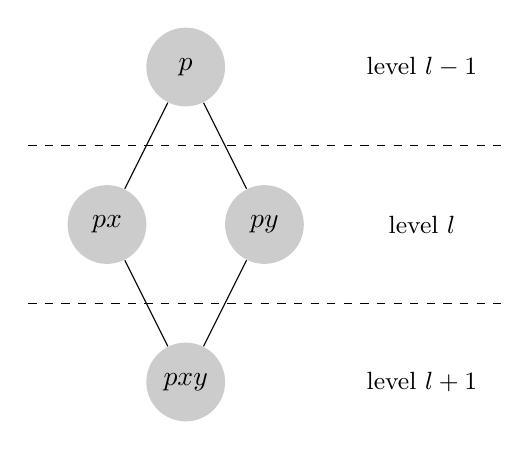
\begin{tikzpicture}
  [scale=1,auto=center,every node/.style={minimum size=1cm}]
    \node (p)  [circle,fill=black!20] at (4,10) {$p$};
    \node (n1) [circle,fill=black!20] at (3,8)  {$p x$};
    \node (n2) [circle,fill=black!20] at (5,8)  {$p y$};
    \node (n12)[circle,fill=black!20] at (4,6)  {$p x y$};


    \foreach \from/\to in {p/n1,p/n2,n1/n12,n2/n12}
      \draw (\from) -- (\to);

    \draw[dashed] (2,9) -- (8,9);
    \draw[dashed] (2,7) -- (8,7);

    \node (level0)[font=\small] at (7,10) {level $l-1$};
    \node (level1)[font=\small] at (7,8)  {level $l$};
    \node (level2)[font=\small] at (7,6)  {level $l+1$};
  \end{tikzpicture}
  \label{fig:joinIndepExample}
\end{figure}

Each node $p$ contains a histogram $h(p)$ with the example frequencies and we define $h_i(p)$ as the frequency of bucket
$b_i$ in $h(p)$. For the example shown in figure \ref{fig:joinIndepExample}, we can calculate the conditional
probability $p_i(x|p)$ and $p_i(y|p)$. With that, we can calculate $\hat{h_i}(p x y)$, which is the estimation of
$h_i(p x y)$ assuming that $x$ and $y$ are independent given common parent $p$.

\begin{equation}
\label{eq:condindep}
\begin{split}
 p_i(x|py) &= p_i(x|p) \\ 
 &= \cfrac{h_i(xp)}{h_i(p)} \\ 
 p_i(y|px) &= p_i(y|p) \\ 
 &= \cfrac{h_i(yp)}{h_i(p)} \\ \\ 
 \hat{h_i}(pxy) &= p_i(x|py)p_i(y|p)*h_i(p) \\ 
 &= p_i(x|p)h_i(yp) \\ 
 \hat{h_i}(pxy) &= p_i(y|px)p_i(x|p)*h_i(p) \\ 
 &= p_i(y|p)h_i(xp) 
\end{split}
\end{equation}

After that, we query the actual frequency distribution on the knowledge base and do a Pearson's chi-squared
independence test. As null hypothesis and alternative hypothesis we have:

\begin{itemize}
 \item $H_0$ = \emph{$x$ and $y$ are conditionally independent given their common parent $p$}
 \item $H_1$ = \emph{$x$ and $y$ are conditionally dependent given their common parent $p$} 
\end{itemize}

Number of degrees of freedom is the number of buckets minus one:

\begin{center}
 $df=k-1$
\end{center}

We calculate the critical value $\chi^2$:

\begin{equation}
 \chi^2=\sum_{i=1}^{k} \cfrac{(h_i - \hat{h_i})^2}{\hat{h_i}}
\end{equation}

\cite{Jaroszewicz02pruningredundant}

Then it's possible to obtain the p-value and check whether there's enough confidence to reject the null hypothesis
$H_0$. 


In other words if we find out that $x$ and $y$ are conditionally independent given $p$, we could rewrite the equation
\ref{eq:condindep} as the following rules being equivalents, with similar accuracy distributions:

\begin{center}
  $x \leftarrow py \equiv x \leftarrow p $ \newline 
  $y \leftarrow px \equiv y \leftarrow p $
\end{center}

Therefore, we know that if we have $x$ fixed as head of clauses in the core ILP, and we currently have $x \leftarrow p$
joining the node $px$ with $py$ to obtain the rule $x \leftarrow py$ does not add any valuable information. The same
applies
for having $y$, and obtaining $y \leftarrow px$ from $y \leftarrow p$ by joining the same pair of nodes. This property
plays an important role in the integration of the correlation lattice into the core ILP as we will explain in more
details later in Section (???).

Nevertheless it cannot be safely pruned from the lattice.  

\begin{comment}
In level 1 from \graphname, nodes can be directly pruned, on the other hand, for further levels, for a node to be
pruned by independence, all the possible joins resulting the node must be independent. In level 2, for example, in order
to prune the node $r a_1 b_1 c_1$, given that in level 1 the nodes $r a_1 b_1$, $r a_1 c_1$ and $r b_1 c_1$ were not
pruned. All the three possible join combinations should fail the independence test, i.e.:

\begin{equation}
\begin{split} 
  freq(r a_1 b_1 c_1) &\approx freq(r a_1)p (r b_1|r a_1) p(r c_1|r a_1) \\ 
  &\approx  freq(r b_1) p(r a_1|r b_1) p(r c_1|r b_1) \\ 
  &\approx  freq(r c_1) p(r a_1|r c_1) p(r b_1|r c_1)  
\end{split}
\end{equation}
\end{comment}

This applies to nodes at any level $l$, with $p \leq l$ parents and $C_{2}^{p}$ possible join pairs. If any of the join
pairs has enough evidence of being dependent, then 2 edges are created connecting each of the joined
nodes to the result of their join

\subsection{Entropy Divergence Measures}

As seen in the previous sections, we are interested in rules whose base-rule has accuracy below threshold, but contains
one or multiple specific intervals with accuracy above threshold. For this to happen, we need a rule with non-uniform
accuracy distribution, or in other words, divergent body support and rule positive examples distributions.

Therefore, we are interested in adding categories that produces distributions different from their parent nodes'. In
order to measure such divergence between distributions, some of the state-of-the-art such as the following ones can be
used.

\begin{itemize}
 \item Kullback-Leibler \cite{Kullback51klDivergence}: 
    \begin{equation}
      D_{KL}(P||Q)=\sum_{\substack{i}}\ln\left(\cfrac{P(i)}{Q(i)}\right)*P(i)
    \end{equation}
 \item Chi-squared ($\chi^2$):
    \begin{equation}
      D_{\chi^2}(P||Q)=\sum_{\substack{i}}\cfrac{(P(i)-Q(i))^2}{P(i)}
    \end{equation}
 \item Jensen-Shannon \cite{17795}:
    \begin{equation}
      D_{JS}(P||Q)=\cfrac{1}{2}D_{KL}(P||M)+\cfrac{1}{2}D_{KL}(Q||M), 
    \end{equation}
\end{itemize}

Where $P$ and $Q$ are discrete distributions to be compared and $M=\cfrac{1}{2}(P+Q)$. In the lattice context, these
distributions would be the frequency histogram normalized to 1, and nodes directly connected by edges would have their
distributions compared.

As discussed in \cite{17795}, although Jensen-Shannon is computationally more expensive, it has the advantage of being a
symmetric and smoothed version of the Kullback-Leibler measure.

These divergence measures are important for identifying potential accuracy distributions. If the divergence between the
frequency distributions of a parent and child node is big, that means that if we have a rule with the parent node as
body and the additional literal from the child as head, its accuracy distribution will be not uniform and therefore
potentially interesting for searching for refined-rules with numerical intervals.


\subsection{Heuristics}

As seen before, the number of nodes in \graphname grows exponentially with the number of categorical relations
and its constants. For $n$ categorical relations, each with $m$ constants, the total number of nodes is $2^{nm}$. As we
limit the number of levels in the lattice to $l$, the total number of nodes reduces to:

\begin{center}
  \begin{equation}
    \sum_{i=1}^{l}\binom{nm}{i}
  \end{equation}
\end{center}

if $l=nm$:

\begin{center}
  \begin{equation}
    \sum_{i=1}^{mn}\binom{nm}{i} = 2^{nm}
  \end{equation}
\end{center}


Pruning by support is usually not sufficient to make it feasible and it's necessary to apply
heuristics to prune it more aggressively.

%%% Divergence

Pruning by divergence is clearly not safe. Let's suppose we have a root numerical property $r(x,y)$, and two categorical
relations $a(x,z)$ with constants $A_1$ and $A_2$ and $b(x,w)$ with constants $B_1$ and $B_2$. For simplicity, let's
assume y is divided in two buckets and root $r$ has an uniform distribution $[0.5 \, 0.5]$ from frequencies $[2 \, 2]$.
It's possible to have $r a_1$ and $r a_2$ as well as $r b_1$ and $r b_2$ with the same uniform distribution with
frequencies $[1 \, 1]$. Nevertheless when combined we can have the following:

$r a_1 b_1 : [1.0 \, 0.0] \\$
$r a_1 b_2 : [0.0 \, 1.0] \\$
$r a_2 b_1 : [0.0 \, 1.0] \\$
$r a_2 b_2 : [1.0 \, 0.0]$

As shown above, divergence is not a monotonically decreasing measure, thus it can only be used as heuristics.

% Draw example instead to explain better

Moreover, using a divergence measure alone might also be problematic. Histograms with low support are more likely to
present a higher divergence than histograms with higher support, supposing that they were drawn from the same original
distribution. Consequently, and algorithm using only the divergence as heuristics would end up giving preference to
nodes with lower support. Therefore, it's important to use divergence combined with support as pruning heuristics.
[Restructure, it's confusing]

%Moreover, we are interested not only in rules with high confidence, but also rules with high support so more facts can
%be derived.

% Talk about how to use such measure? (Threshold, Top-k, Cost-Benefit)

%%% Independence

As seen seen in Section (???), checking for conditional independence of categories is very insightful and
can detect equivalent rules like in Figure \ref{fig:joinIndepExample} where we know that 
$x \leftarrow py \equiv x \leftarrow p$ and $y \leftarrow px \equiv y \leftarrow p$. Nevertheless, we cannot prune the
node $pxy$ from the lattice as we $x$ and $y$ might not be independent given $pz$, and for instance, a rule $x
\leftarrow pyz$ might not be equivalent to $x \leftarrow py$. 

\section{Bucketing Numerical Attributes}

So far we have mentioned that the root's numerical attribute domain should be discretized by dividing it in buckets in
order to build frequency histograms and compare distributions. In this section, we will discuss about how to perform
such discretization.

The buckets used throughout the \graphname should be consistent, and the bucketing method as well as the boundaries are
specified in the very beginning with the root node. It should have as input an arbitrarily defined number of buckets
$k$.

\subsection{Bucketing by Domain}
This bucketing method consists of simply querying both the maximum and minimum value of the root's numerical attribute
and 

\subsection{Bucketing by Support}


\section{Incorporating \graphname into the Core ILP Algorithm}

The ILP core learning algorithm requires some modifications in order to support the \graphname. As stated before, we use
the top-down search, starting from the most general clauses then further refining them by introducing new substitutions
or literals until stopping criteria is reached.

[...]

\subsection{Querying the \graphname}

In the ILP there's a fixed head literal and such literal can and should be included in the \graphname. In case it's
present in the lattice, it plays a key role in the search. Once the root property is added in a clause that does not
exceed the accuracy threshold.

In such case we are interested in searching the most interesting literals to add. First step would be to search in the
lattice the literals already present in both head and body of the clause that are joined with the root. Nevertheless,
what we are not really interested in the benefit of adding a literal to the conjunction of rule's head and body, but in
the benefit of adding the head to a body with a new literal.

For example, if we have the clause $a \leftarrow r$, $r$ is the root of a \graphname and the head $a$ is included in it.
After searching in the graph for the literals joined with root present in the clause we would come to node
$ra$. We are not searching for the most interesting child from $ra$, but for the children, which has a parent without
the head literal that has the has the highest interestingness measure when adding the head.

\begin{figure}[!h]
  \caption{Node join example for independence test}
  \centering
  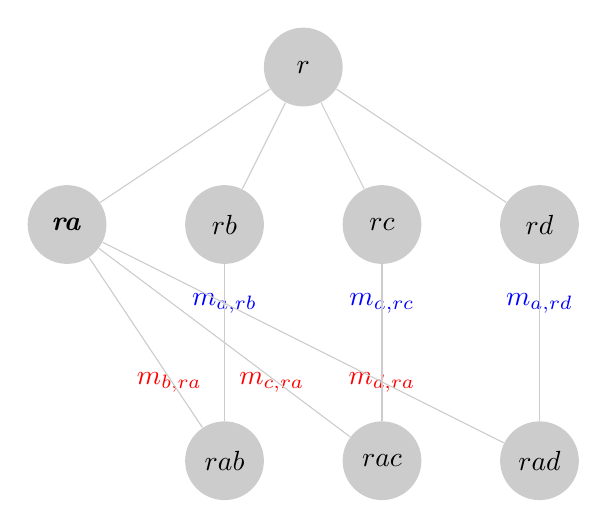
\begin{tikzpicture}
  [scale=1,auto=center,every node/.style={minimum size=1cm}]
    \node (r)  [circle,fill=black!20] at (4,10) {$r$};
    \node (ra) [circle,fill=black!20] at (1,8)  {\textbf{\emph{ra}}};
    \node (rb) [circle,fill=black!20] at (3,8)  {$r b$};
    \node (rc) [circle,fill=black!20] at (5,8)  {$r c$};
    \node (rd) [circle,fill=black!20] at (7,8)  {$r d$};
    \node (rab)[circle,fill=black!20] at (3,5)  {$r a b$};
    \node (rac)[circle,fill=black!20] at (5,5)  {$r a c$};
    \node (rad)[circle,fill=black!20] at (7,5)  {$r a d$};

    \node (m1)[blue] at (3,7)  {$m_{a,rb}$};
    \node (m2)[blue] at (5,7)  {$m_{a,rc}$};
    \node (m3)[blue] at (7,7)  {$m_{a,rd}$};
    \node (m4)[red] at (2.3,6)  {$m_{b,ra}$};
    \node (m5)[red] at (3.6,6)  {$m_{c,ra}$};
    \node (m6)[red] at (5.0,6)  {$m_{d,ra}$};



    \foreach \from/\to in {r/ra,r/rb,r/rc,r/rd,ra/rab,ra/rac,ra/rad,rb/rab,rc/rac,rd/rad}
      \draw[black!20] (\from) -- (\to);

    %\draw (ra) -- (rab) -|  \node [below,pos=0.25] {$m_1$}(l1);
  \end{tikzpicture}
  \label{fig:latticeSuggestion}
\end{figure}

As shown in Figure \ref{fig:latticeSuggestion}, if we can add $b$, $c$ or $d$ to $ra$, we are interested about the
measures in blue instead of the ones in red. Nevertheless, searching for values for $m_{a,rb}$, $m_{a,rc}$ and
$m_{a,rd}$ is a bit tricky. It's necessary to check for all children of $ra$, which ones have parents without head
literal $a$, then gather all the measures and rank them.

In order to make it simpler, we can create a map during lattice build. This map would contain an entry for all node
it's joined to, with head as key and literals to add sorted by measure as value. So for example when we are obtaining
the node $rab$ by joining $ra$ and $rb$, we add to $ra$ an entry with $a$ as key, $b$ as new literal and
associated measure $m_{a,rb}$ and we also add to $rb$ an entry with $b$ as key, $a$ as new literal ad associated
measure $m_{b,ra}$. 

In the example of Figure \ref{fig:latticeSuggestion}, $ra$ would contain the following map:

\begin{center}
  \begin{tabular}{r | l}
    a & b [$m_{a,rb}$] \\
      & c [$m_{a,rd}$] \\
      & d [$m_{a,rc}$]
  \end{tabular}
\end{center}

As in this example the node $ra$ has only two literals, and the root $r$ can't be the head, we use the node $ra_1b_1$
in Figure \ref{fig:lattice} to better illustrate it:

\begin{center}
  \begin{tabular}{r | l}
    a1 	& c1 [$m_{a_1,rb_1c_1}$] \\
	& c2 [$m_{a_1,rb_1c_2}$] \\
    \hline
    b1	& c1 [$m_{b_1,ra_1c_1}$] \\
	& c2 [$m_{b_1,ra_1c_2}$]
  \end{tabular}
\end{center}

In a node at level $l$ with $l+1$ literals (one being the root), we can have up to $l$ keys in the map. Therewith, we
can much more easily find the best suggestions for any possible head literal without having to visit other nodes.

First we need to introduce a new refinement operator that extracts the support and accuracy distributions along a chosen
numerical property and searches for interesting ranges. With that there are

\begin{algorithm}[!h]
 \caption{Refinement step}
 \label{alg4}
 \SetKwFunction{checkNumericalRanges}
 \KwIn{\textbf{Input:} $clause$: Set of literals from the clause, $lattice(r_{root})$: Set of existent Correlation Lattices, 
 $lit_{body}$: Literal in clause that will be joined with new Literal, $lit_{new}$: Literal to be added to the clause,
 $arg_{body}$: Join argument from body literal, $arg_{new}$: Join argument from new literal \\}
 \KwOut{True if $arg_i$ from $r_i$ joins with $arg_j$ from $r_j$, False otherwise}
 
  $r_{new} \leftarrow lit_{new}.relation$ \;
  \If{$arg_{new} = 1$ \textbf{and} $r_{new}$ is numerical \textbf{and} $\exists$ $lattice(r_{new})$} {
    $node \leftarrow$ $lattice(r_{new}).root$.\FuncSty{search(}$head$\FuncSty{)} \;
    \ForEach{$lit_i \in clause.body$} {
      $node \leftarrow node$.\FuncSty{search(}$lit_i$\FuncSty{)} \;
    }
    \FuncSty{checkNumericalRanges(}$clause$,$lit_{new}$,$node$\FuncSty{)} \;
  }
\end{algorithm}

\begin{algorithm}[!h]
 \caption{checkNumericalRanges}
 \label{alg4}
 \SetKwFunction{queryAccuracyDistribution, querySupportDistribution}
 \KwIn{\textbf{Input:}  \\}
 \KwOut{}
  $v \leftarrow $ Numerical variable from $lit_{new}$ \;
  $acc \leftarrow $ \FuncSty{queryAccuracyDistribution(}$clause$,$v$\FuncSty{)} \;
  $sup \leftarrow $ \FuncSty{querySupportDistribution(}$clause$, $v$\FuncSty{)} \;
  $intervals \leftarrow $  \FuncSty{searchInterestingIntervals(}$acc$,$sup$,$accTS$,$supTS$\FuncSty{)} \;
  \ForEach{$interval_i \in intervals$} {
     $newClause \leftarrow \{clause \cup lit_{new} \cup \{v \in interval_i\}\}$ \;
     Add $newClause$ to rule tree \;
  }
  $suggestions \leftarrow node.getSuggestions(clause.head)$ \;
  \ForEach{$lit_i \in suggestions$ \textbf{and} $i \leq k$} {
    $node_i \leftarrow node$.\FuncSty{search(}$lit_i$\FuncSty{)} \;
    \FuncSty{checkNumericalRanges(}$clause \cup lit_i$,$lit_{new}$,$node_i$\FuncSty{)} \;
  }
\end{algorithm}

In the specialization step, we can detect whether the clause contains any numerical property, which is root of a
\graphname. If so, it can search for interesting numerical ranges and combine them with the best , 

